The far field amplitudes is shown to be
\[
    A_j^{\pm \infty} = \mp \int_{S_{\mathrm{B}}} \big( \kappa \phi_j \nhat^{\ast} + i\hat{n}_j \big) e^{\kappa(y \pm ix)} \,\dee S.
\]
The added mass and damping coefficients are found by taking the real and imaginary parts of the integral
\[
    \int_{S_{\mathrm{B}}} \phi_j \hat{n}_i \,\dee S.
\]
Consulting the course notes, we furthermore have that the damping may be approximated by
\[
    r_{22} = \frac{\varrho \omega}{2} \left( {\absl{A^{\infty}_{2}}}^2 + {\absl{A^{-\infty}_{2}}}^2 \right).
\]
\begin{Figure}
    \centering
    \captionsetup{type = figure}
    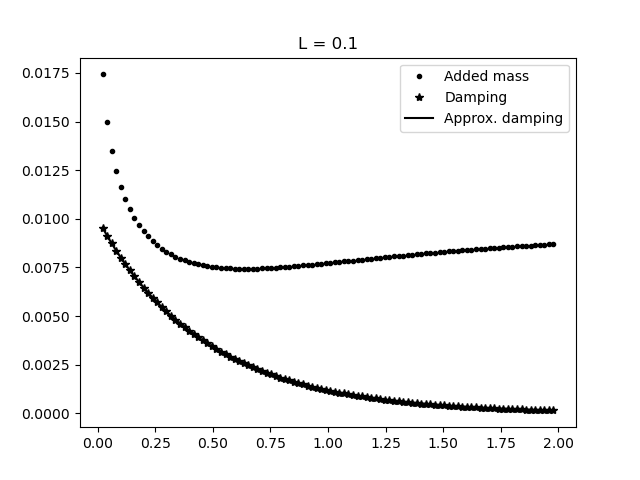
\includegraphics[width = \textwidth]{added_mass_Lp1.png}
    \caption{Added mass for $\sfrac{L}{D} = 0.1$.}
\end{Figure}
\begin{Figure}
    \centering
    \captionsetup{type = figure}
    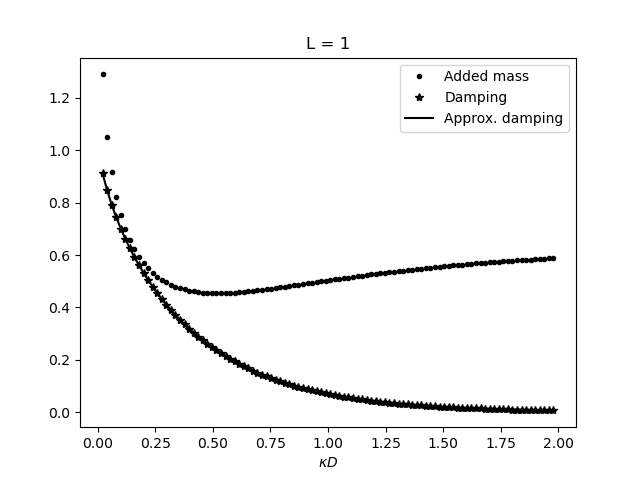
\includegraphics[width = \textwidth]{added_mass_L1.png}
    \caption{Added mass for $\sfrac{L}{D} = 1$.}
\end{Figure}
\begin{Figure}
    \centering
    \captionsetup{type = figure}
    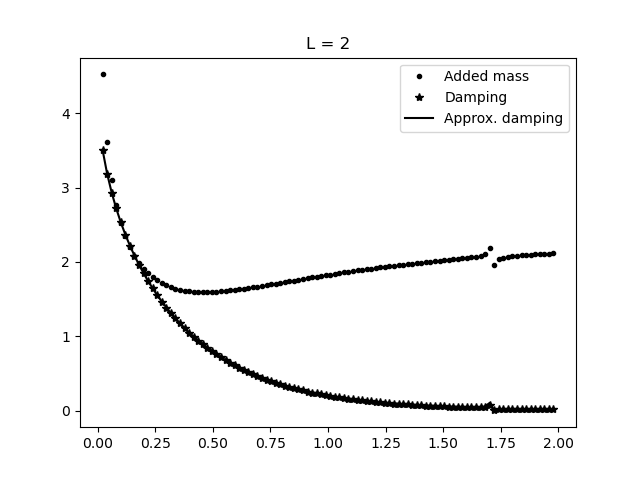
\includegraphics[width = \textwidth]{added_mass_L2.png}
    \caption{Added mass for $\sfrac{L}{D} = 2$}
\end{Figure}
\begin{Figure}
    \centering
    \captionsetup{type = figure}
    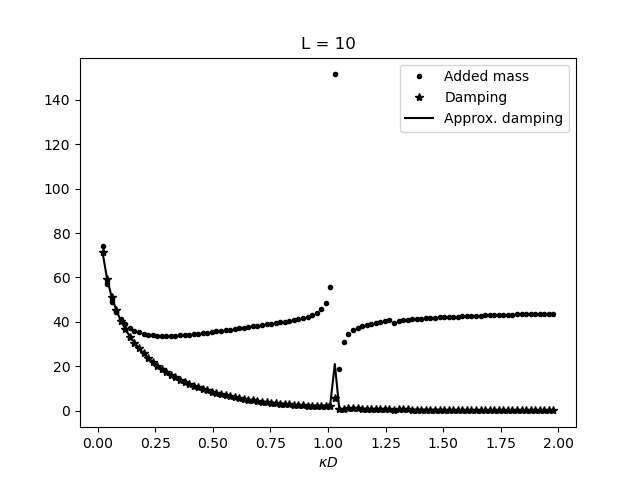
\includegraphics[width = \textwidth]{added_mass_L10.png}
    \caption{Added mass for $\sfrac{L}{D} = 10$.}
\end{Figure}